\documentclass[a4paper]{fhnwreport}
\usepackage{pdfpages}
%\usepackage{float}

\graphicspath{{./graphics/}{./Anhang/}}	
\begin{document}

\subsection{Schaltregler}\label{schaltregler}

Gemäss Vorgaben des Auftraggebers wurde das zur Spannungsregelung zuständige Bauteil mittels eines Abwärtswandlers im Form eines Schaltreglers realisiert. Die Ausgangsspannung des Reglers soll vom Controller in Form einer DC-Spannung reguliert, sodass der Ausgang der im Mikrocontroller Kennlinie entspricht. 

Gewählt wurde der LT1074CT, da dieser Ströme bis zu 5A sowie eine maximale Ausgangsspannung von 50V besitzt. Die maximale Eingansspannung beträgt 60V, deutlich mehr als die Spannung des Netzgerätes, welches 24V liefert.
Des weiteren lässt sich der LT1074CT mittels eines Feedback-Pins regulieren und die TO-220 Gehäuseform erlaubt eine einfache Montage eines Kühlkörpers.

Auch kann bei Bedarf auf den LT1074HVCT gewechselt werden, dieser besitzt nebst den Funktionen des LT1074CT auch noch einen Stromlimit Pin und einen Stutdown Pin. Die Strombegrenzung kann mittels Widerstandes auf einen anderen maximalen Ausgangsstrom als die standardmässigen 6A eingestellt werden. Da jedoch der Strom des Netzteils 3.5A beträgt ist eine Begrenzung des Stromes nicht notwendig und  der Shutdown Pin ist lediglich dazu da um den Regler abzuschalten falls eine zu tiefe Spannung vorhanden ist, weshalb schlussendlich doch für den LT1074CT entschieden worden ist.

\begin{figure}[h]
\centering
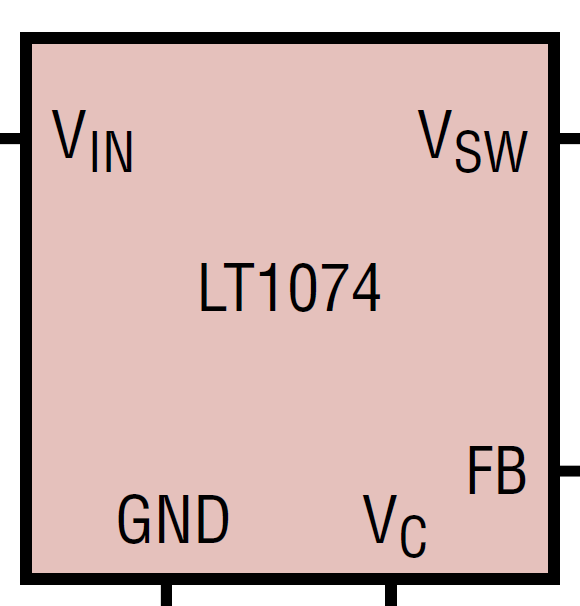
\includegraphics[width=0.2\textwidth]{LTData}%
\caption{Blockschaltbild des LT1074}
\label{fig::LTData}
\end{figure}

Die Schaltung wurde zunächst in LT-Spice simuliert und danach auf einer Lochrasterplatine aufgebaut:

\begin{figure}[h]
\centering
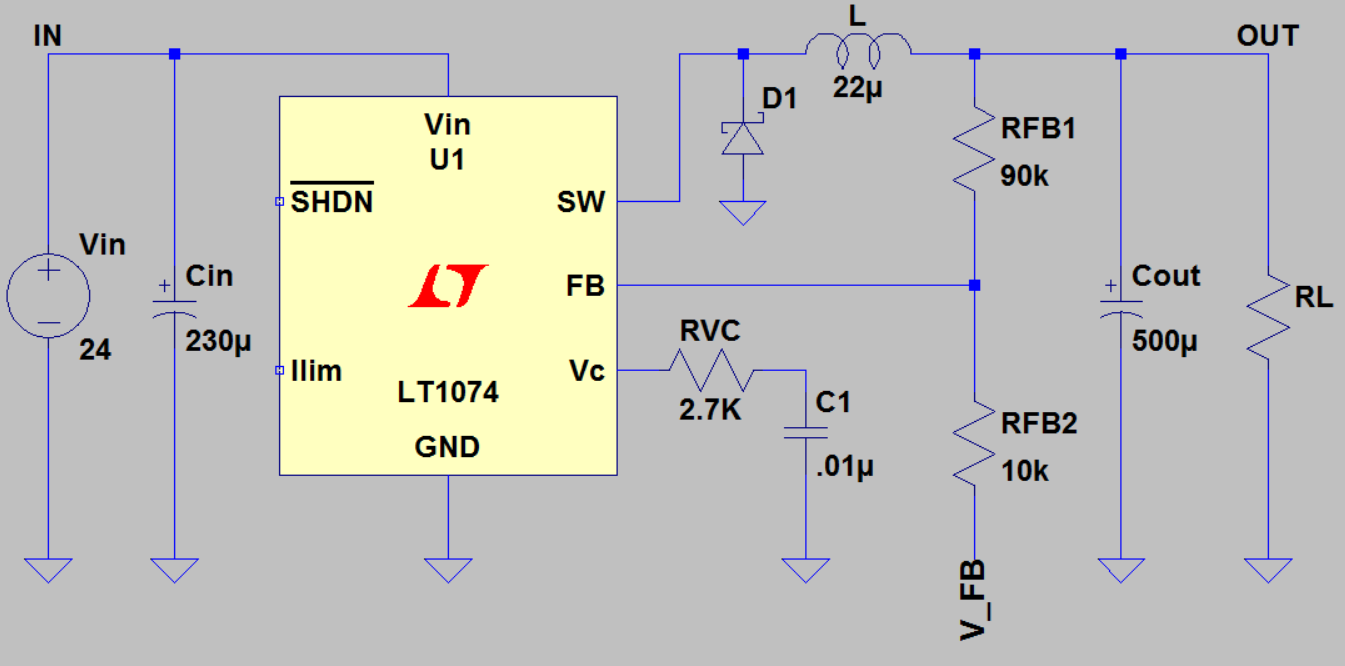
\includegraphics[width=0.8\textwidth]{LTSchemata}%
\caption{Beschaltung des Schaltreglers}%
\label{fig::LTSchemata}%
\end{figure}

Der Widerstand RFB1 wurde nach der folgenden Fromel berechnet:

\[
R_{FB1}=\frac{R_{FB2}\cdot V_{Outmax}}{2.21V}-R_{FB2}
\]

Dabei sind $V_{Outmax} =22$V und $R_{FB2} =10$k$\Omega$, dies ergibt für $R_{FB1} \approx 90$k$\Omega$

Die Spule sowie die Kondensatoren und der Widerstand $R_{Vc}$ wurden gemäss der Appplication Note von Linear Technologies dimensioniert und entsprechen den Empfehlungen des Herstellers.

Mittels der Spannung $V_{FB}$ kann nun die Ausgangsspannung folgendermassen verändert werden:

\[
V_{FB}=2.21\text{V}\cdot\frac{R_{FB1}+R_{FB2}}{R_{FB1}}-V_{out}\cdot\frac{R_{FB2}}{R_{FB1}}
\]

Man sieht sofort das bei einer $V_{FB}$ Spannung von 0V die Spannung maximal wird, das Maximum am Ausgang wird mit einer Spannung von 2.46V erreicht. 

Die Funktion dieser Schaltung wurde im Kapitel \ref{subsec:ValRegler} getestet und validiert.
\end{document}





